\begin{figure}%[t]
\begin{center}
 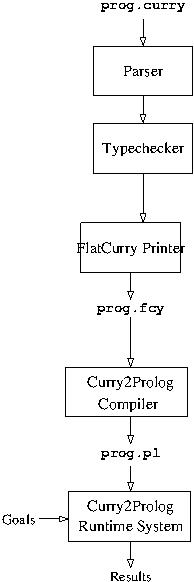
\includegraphics[scale=0.85]{pakcs_overview.jpg}
\end{center}\vspace{-5ex}
\caption{Overview of \CYS\label{fig-pakcs}}
\end{figure}

\section{Overview of the \CYS Distribution}

A schematic overview of the various components contained in
the distribution of \CYS and the
translation process of programs inside \CYS is shown in
Figure~\ref{fig-pakcs} on page~\pageref{fig-pakcs}.
In this figure, boxes denote different components of \CYS
and names in boldface denote files containing
various intermediate representations during the translation
process (see Section~\ref{sec-auxfiles} below).
The \CYS distribution contains a front end for reading (parsing and
type checking) Curry programs that can be also used by
other Curry implementations.
The back end (formerly known as ``Curry2Prolog''\index{Curry2Prolog})
compiles Curry programs into Prolog programs.
It also support constraint solvers for
arithmetic constraints over real numbers and finite domain constraints,
and further libraries for GUI programming, meta-programming etc.
Currently, it does not implement encapsulated search in full generality
(only a strict version of \code{findall} is supported),
and concurrent threads are not executed in a fair manner.


%%% Local Variables: 
%%% mode: latex
%%% TeX-master: "manual"
%%% End: 
